\subsection{What is an operating system?}
Special layer of software that provides application software access to hardware resources
\begin{itemize}
    \item Convenient \textbf{abstraction} of complex hardware devices
    \item Protected access to shared resources
    \item Security and authentication
    \item Communication amongst logical entities
\end{itemize}
\subsection{What Does an OS do?}
\paragraph{Provide abstractions to apps}File systems, Processes, threads, VM, containers, Naming system

\paragraph{Manage resources} Memory, CPU, storage,\dots

\paragraph{Achieves the above by implementing specific algos and techniques}Scheduling, Concurrency, Transactions, Security, \dots

\subsection{Illusionist}
Provide clean, easy-to-use \textbf{abstractions of physical resources}
\begin{itemize}
    \item Infinite memory, dedicated machine
    \item Higher level objects: files, users, messages
    \item Masking limitations, virtualization
\end{itemize}
\begin{figure}[H]
    \centering
    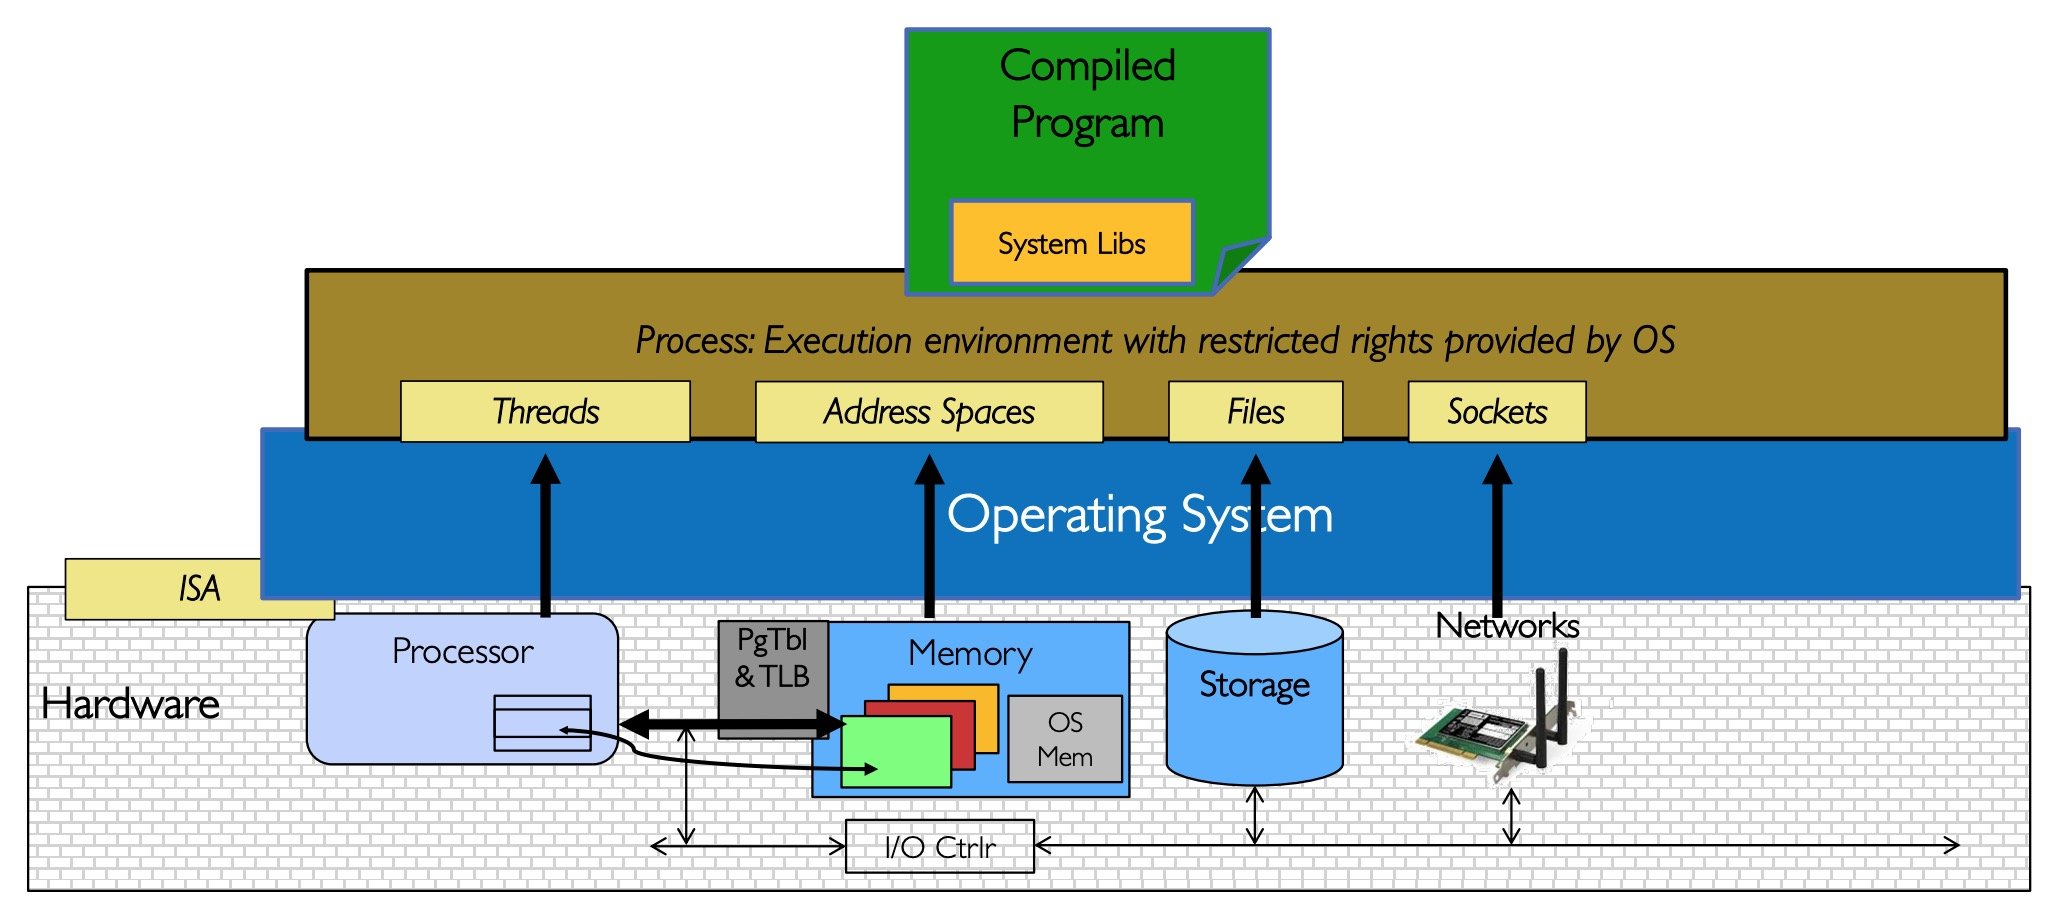
\includegraphics[width = 0.8\textwidth ]{figures/Virtualizing the Machine.jpg}
    \caption{Virtualizing the Machine}
    % \label{fig:batteryIncreas}
\end{figure}

\begin{figure}[H]
    \centering
    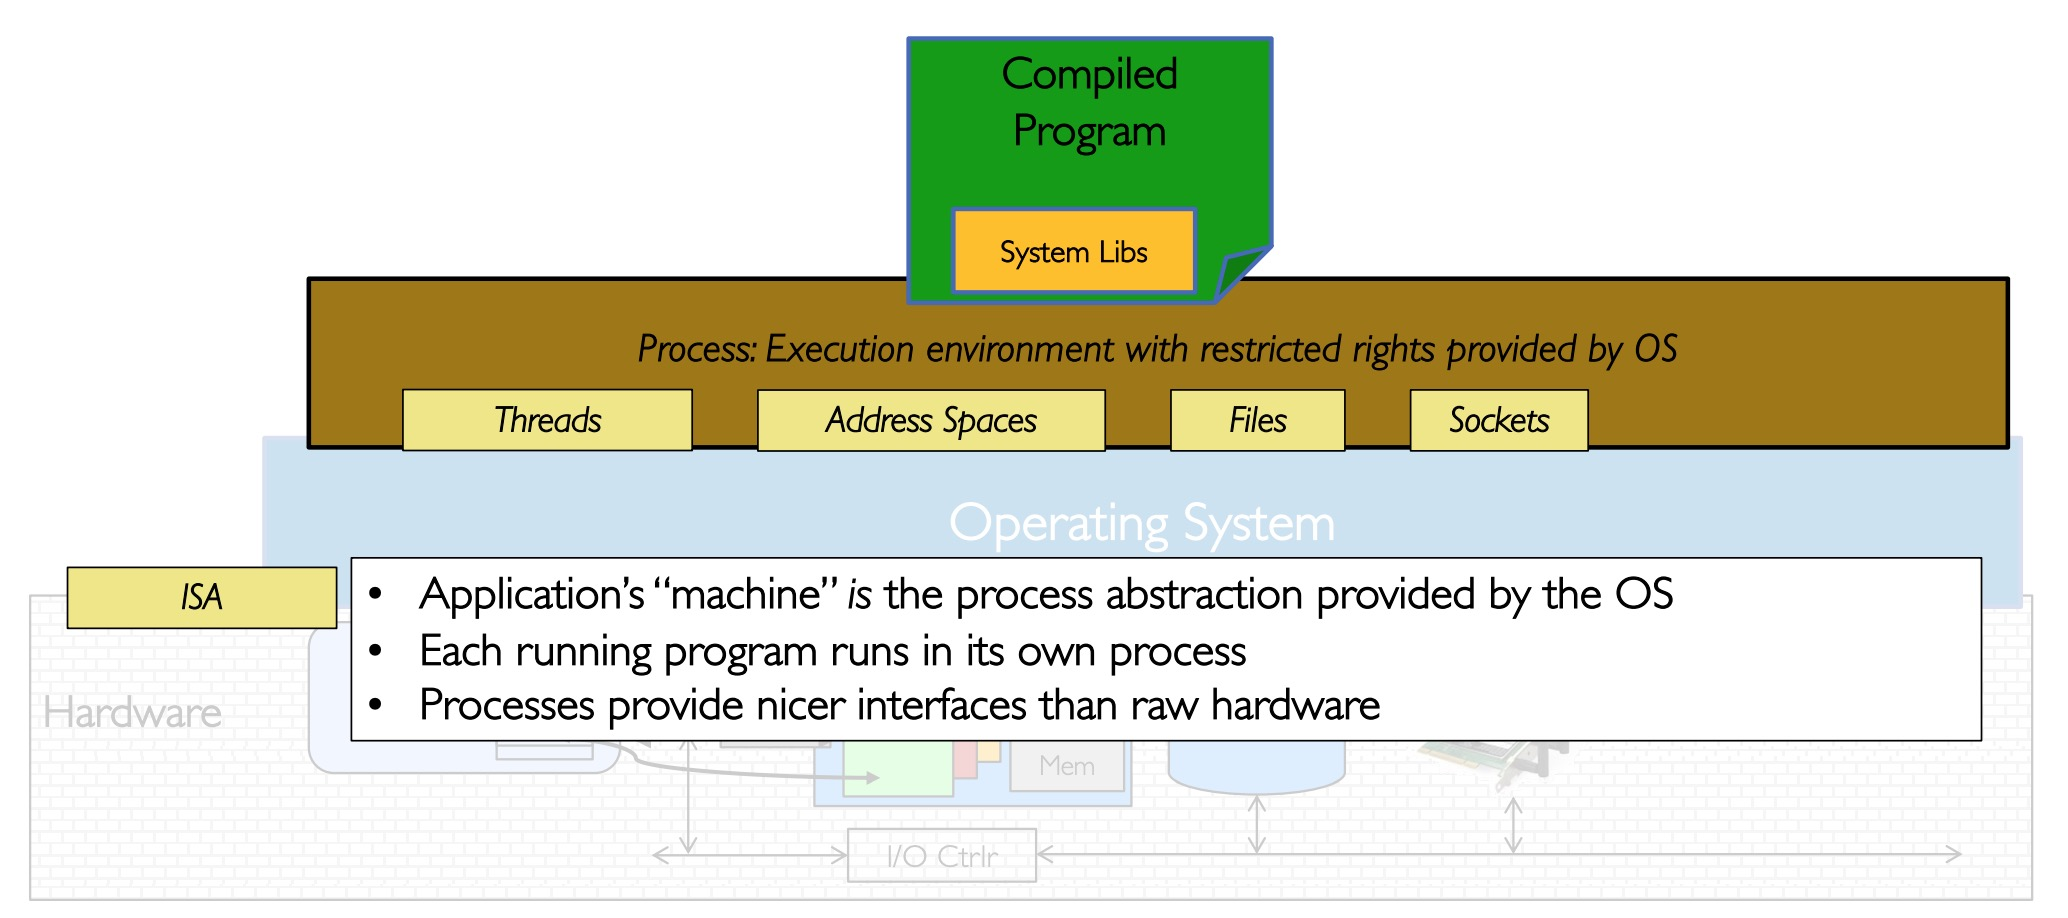
\includegraphics[width = 0.8\textwidth ]{figures/Compiled Program's View of the World.jpg}
    \caption{Compiled Program's View of the World}
    % \label{fig:batteryIncreas}
\end{figure}

\begin{figure}[H]
    \centering
    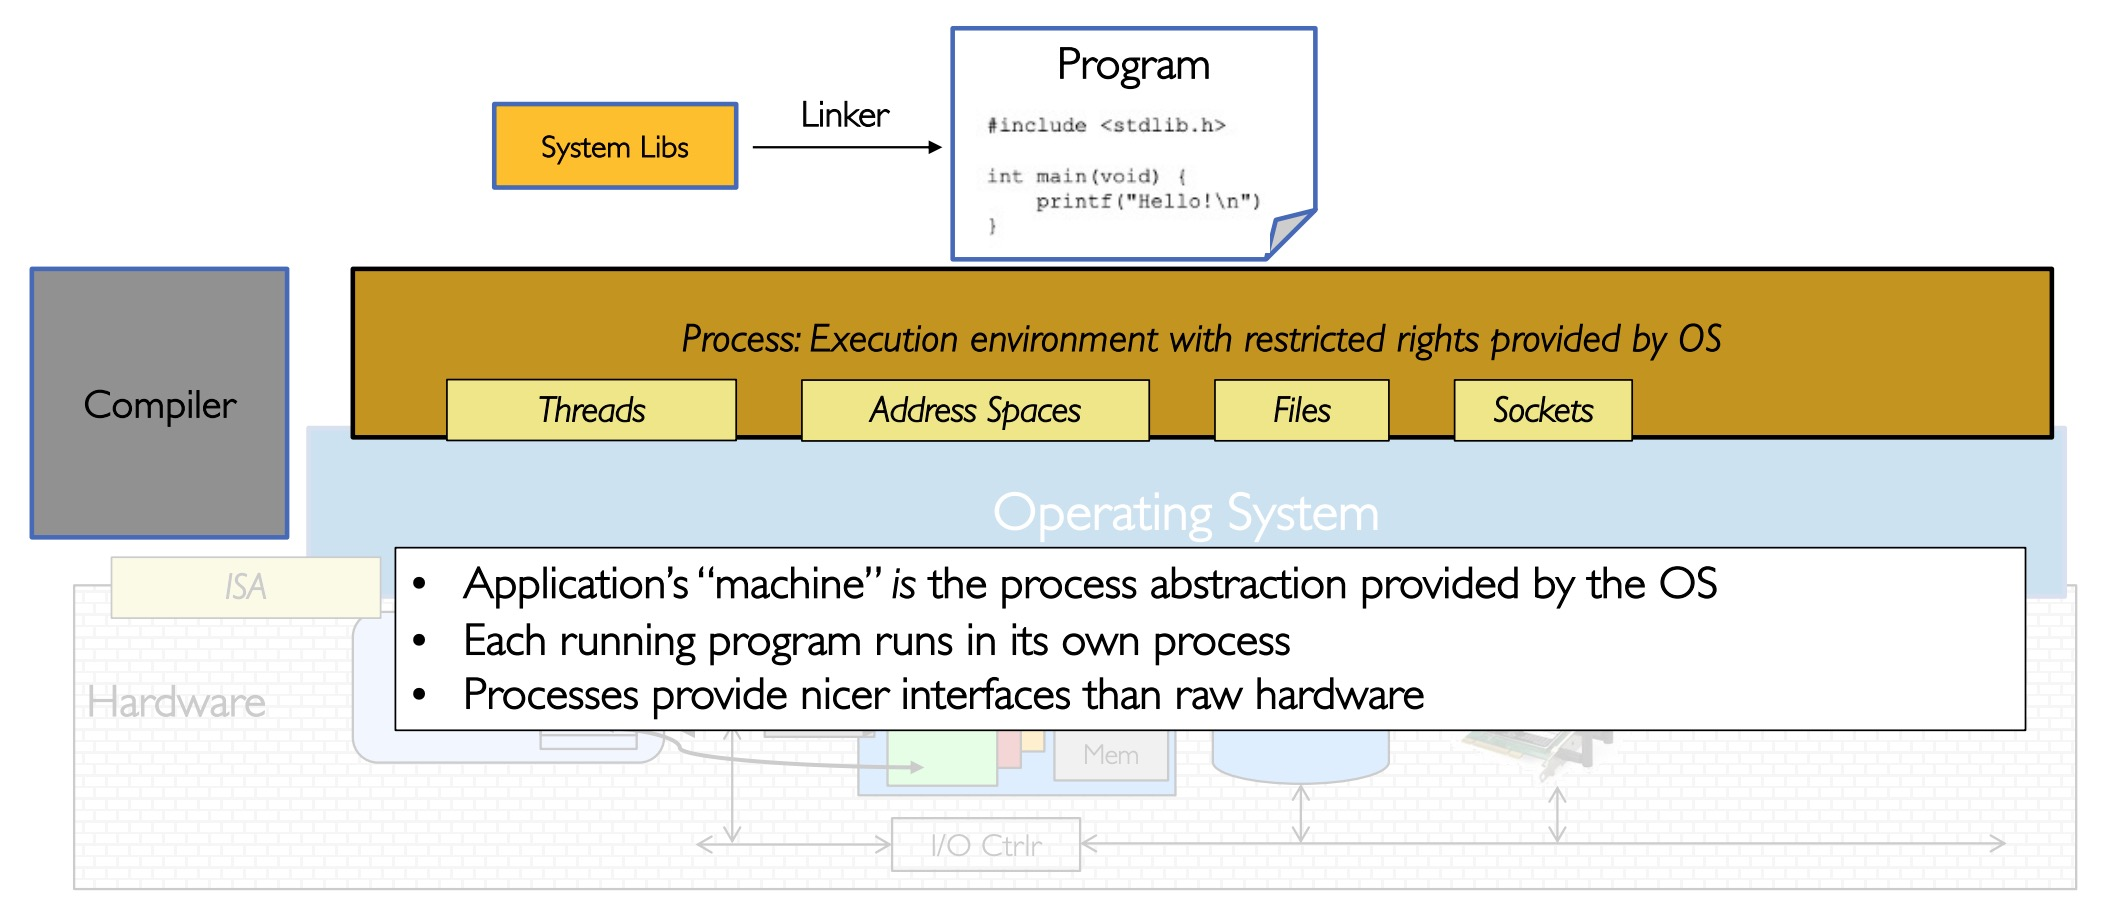
\includegraphics[width = 0.8\textwidth ]{figures/System Programmer's View of the World.jpg}
    \caption{System Programmer's View of the World}
    % \label{fig:batteryIncreas}
\end{figure}
\subsubsection{What's in a Process?}
\noindent A process consists of:
\begin{itemize}
    \item Address Space
    \item One or more threads of control executing in that address space
    \item Additional system state associated with it(Open files, Open sockets)
\end{itemize}
\begin{figure}[H]
    \centering
    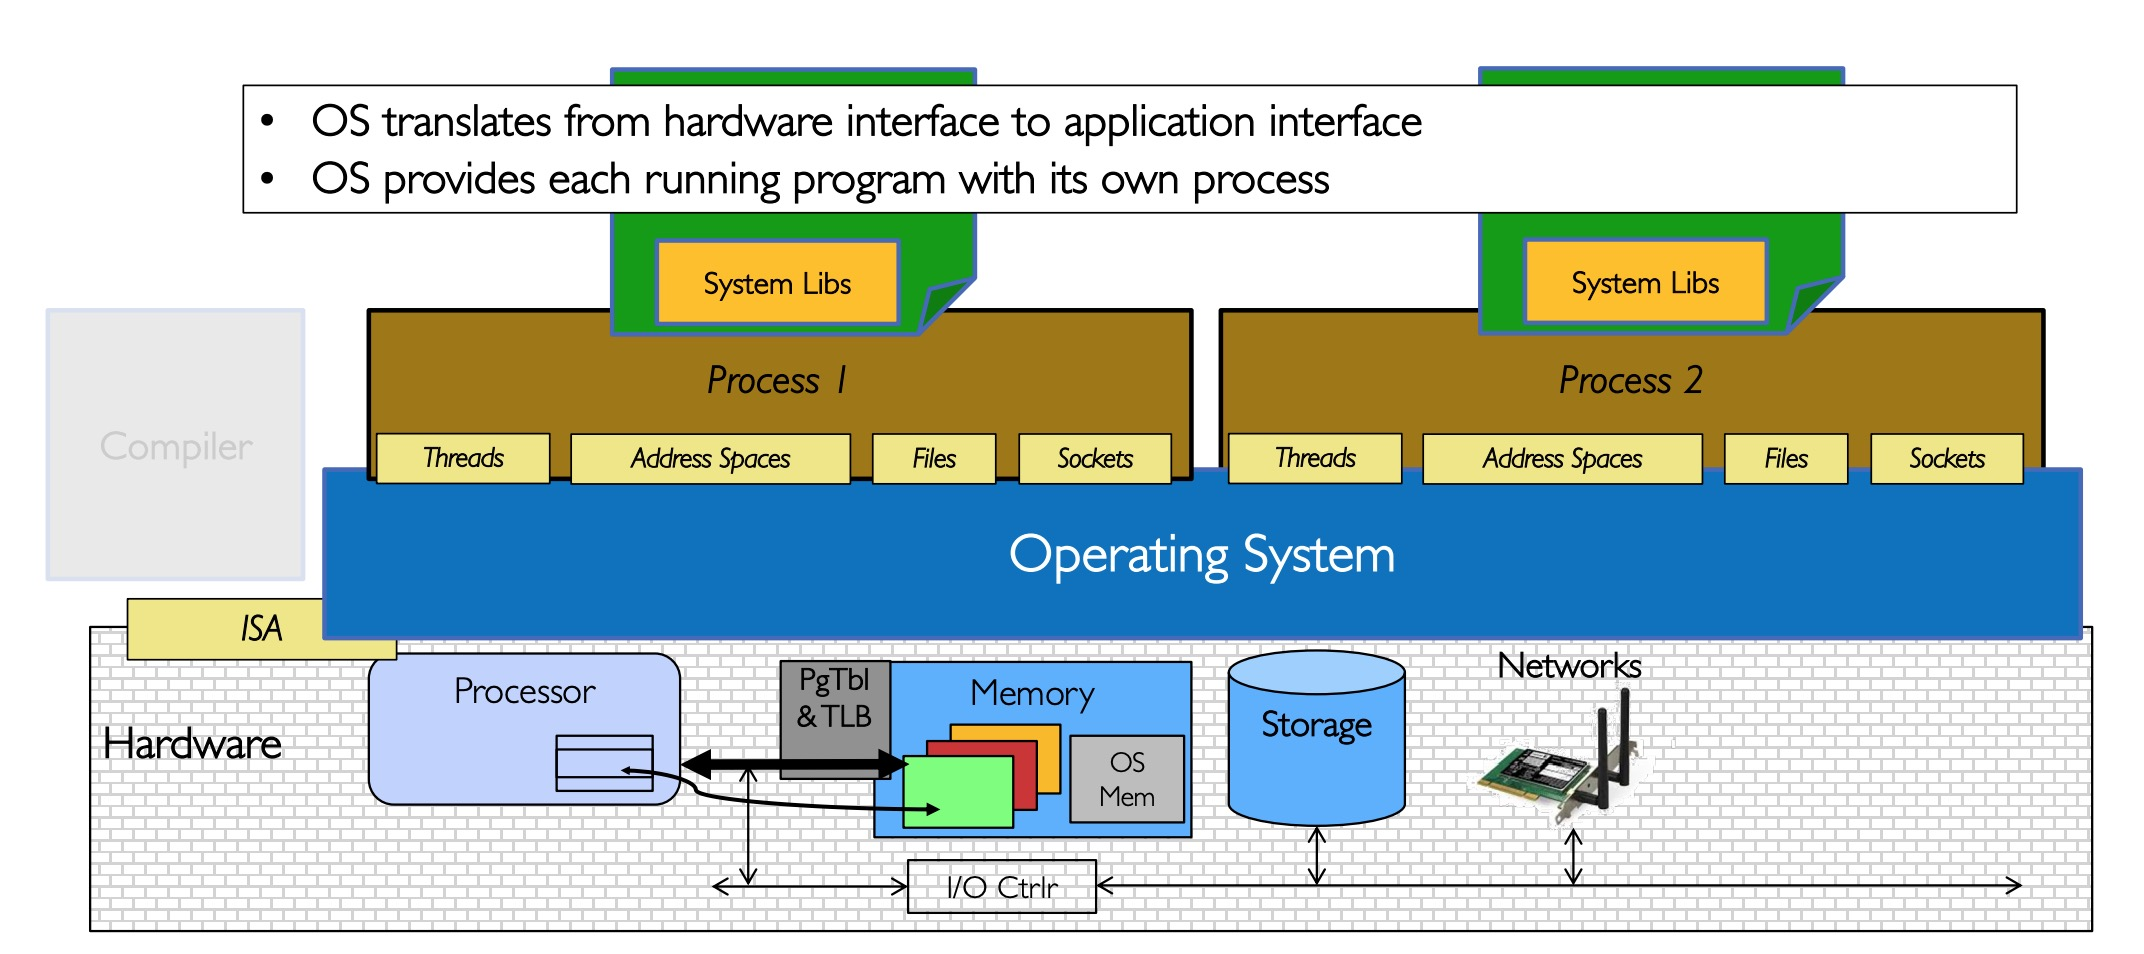
\includegraphics[width = 0.8\textwidth ]{figures/process_in_os_programmer_view.jpg}
    \caption{Process in System Programmer's View}
    % \label{fig:batteryIncreas}
\end{figure}

\subsection{Referee}
Manage \textbf{protection}, \textbf{isolation}, and \textbf{sharing of resources}
\begin{itemize}
    \item Resource allocation and communication
\end{itemize}
\begin{figure}[H]
    \centering
    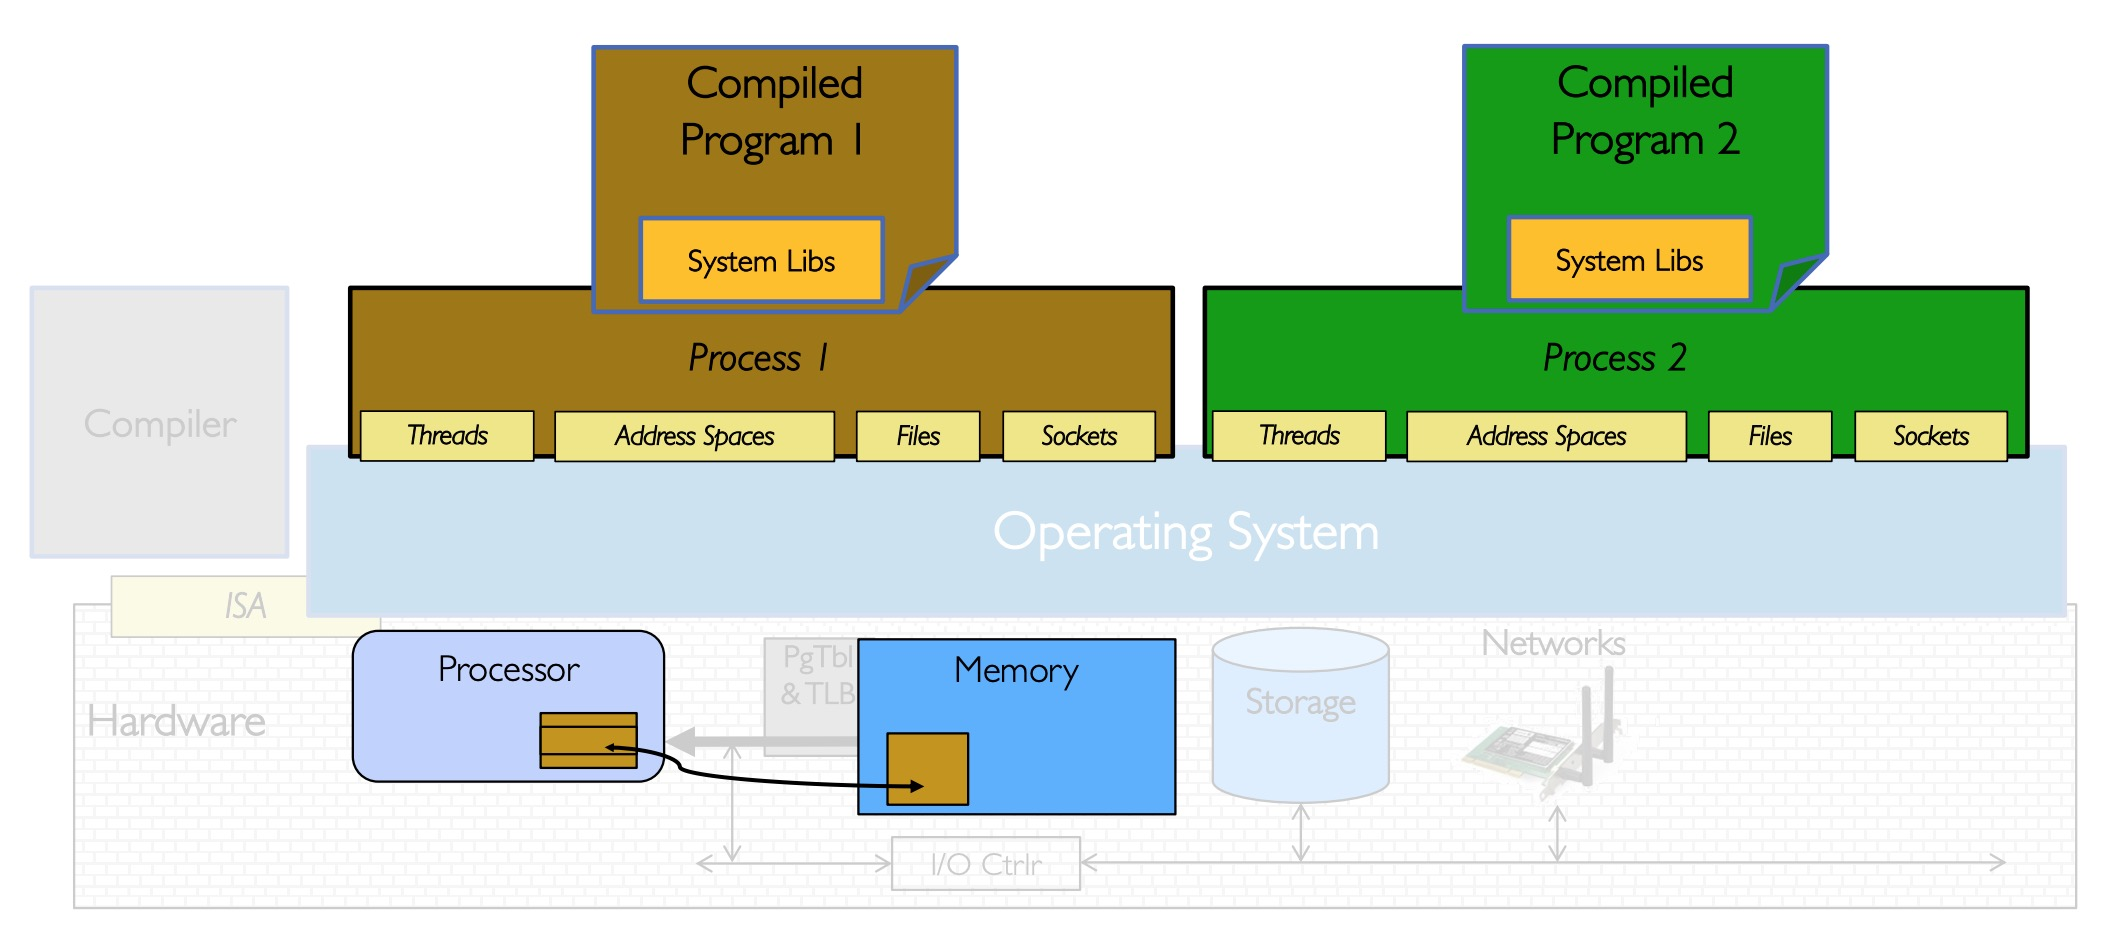
\includegraphics[width = 0.8\textwidth ]{figures/running_process.jpg}
    \caption{Running a Process}
    % \label{fig:batteryIncreas}
\end{figure}

\begin{figure}[H]
    \centering
    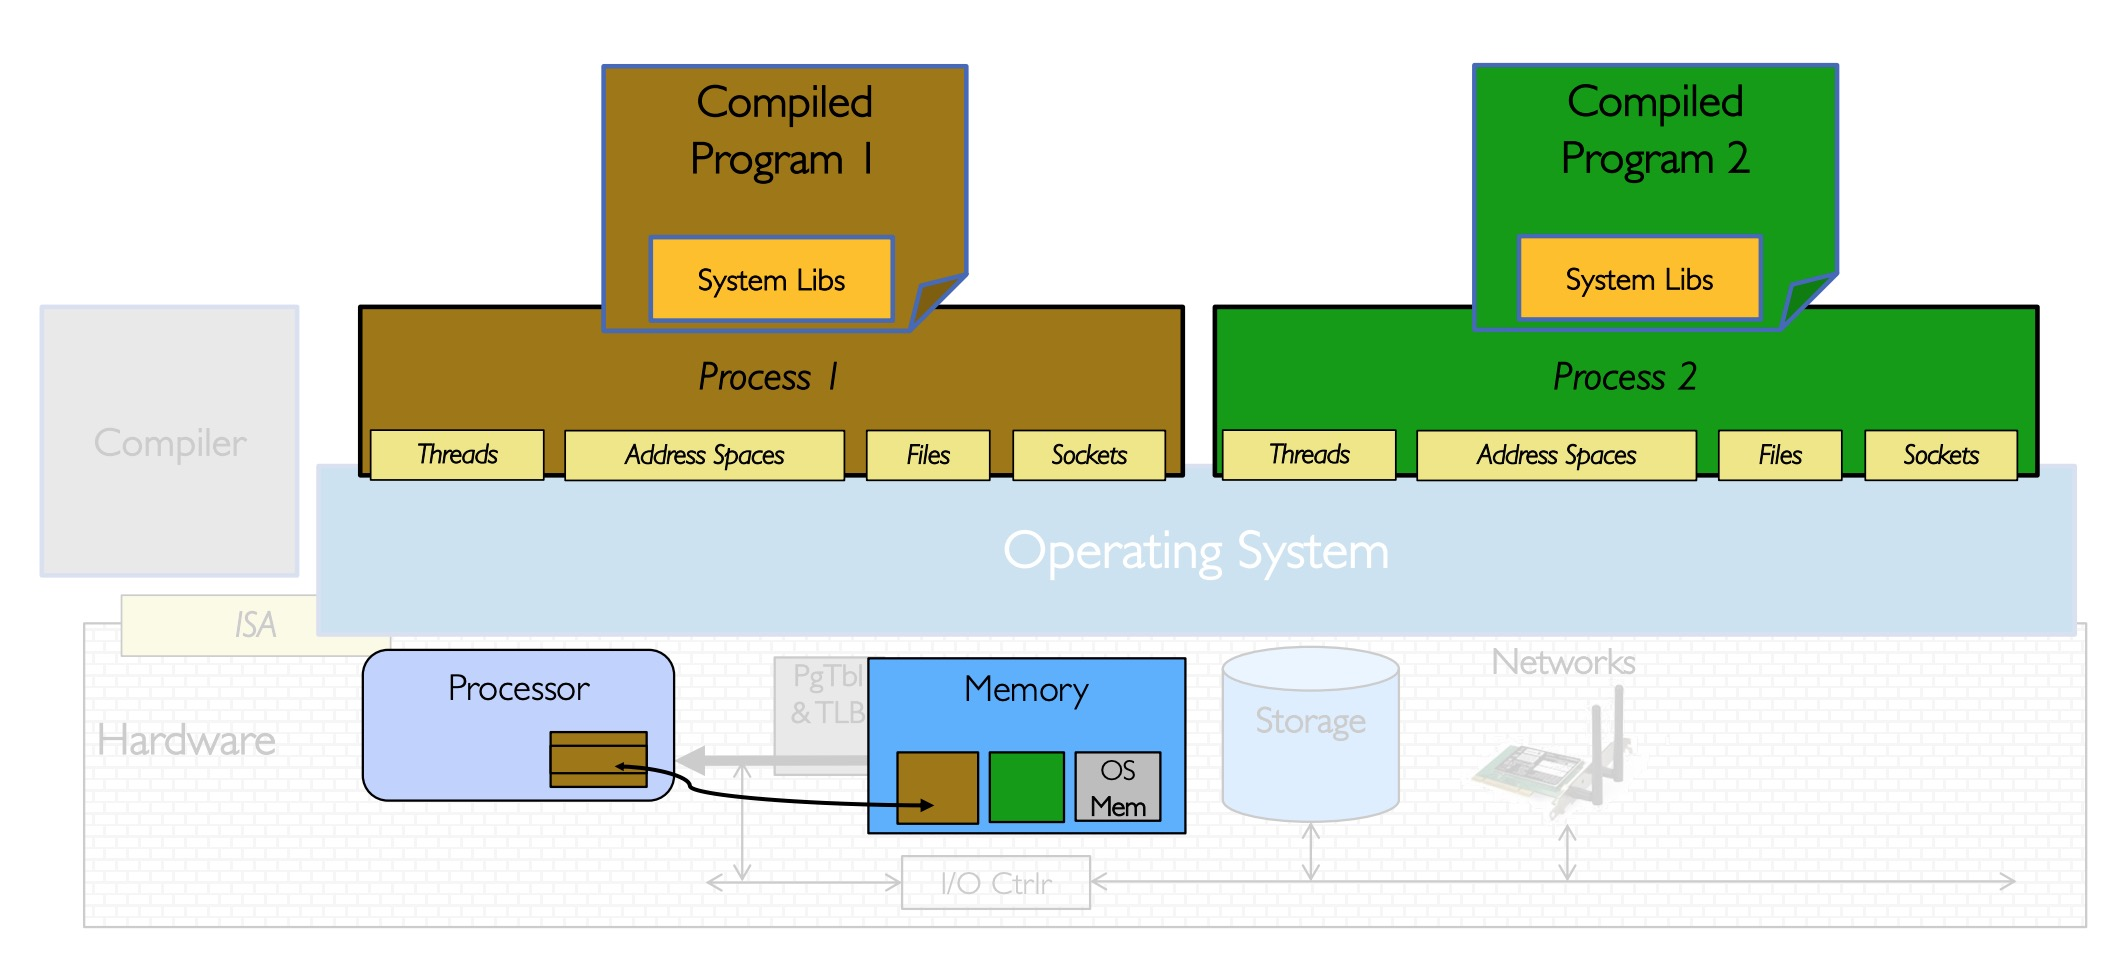
\includegraphics[width = 0.8\textwidth ]{figures/switching_process.jpg}
    \caption{Switching Process 1}
    % \label{fig:batteryIncreas}
\end{figure}
\subsubsection{Protection}
\begin{itemize}
    \item OS \textbf{isolates} processes from each other
    \item OS \textbf{isolates} itself from other processes
\end{itemize}
\begin{figure}[H]
    \centering
    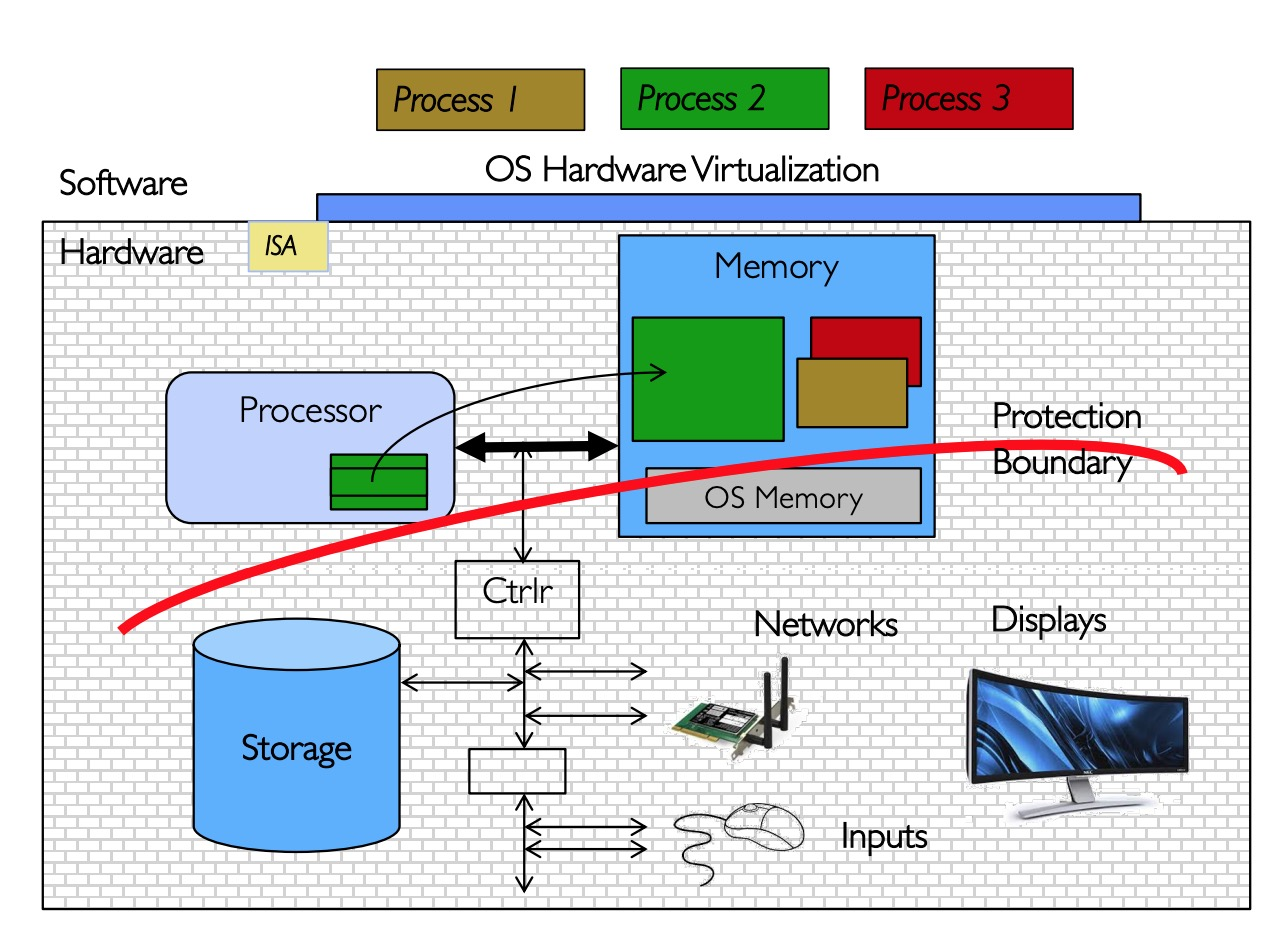
\includegraphics[width = 0.8\textwidth ]{figures/protection.jpg}
    \caption{Protection}
    % \label{fig:batteryIncreas}
\end{figure}

\subsection{Glue}
Common services
\begin{itemize}
    \item Storage, Window system, Networking
    \item Sharing, Authorization
    \item Look and feel
\end{itemize}
\subsubsection{I/O}
OS provides common services in the form of I/O

\begin{figure}[H]
    \centering
    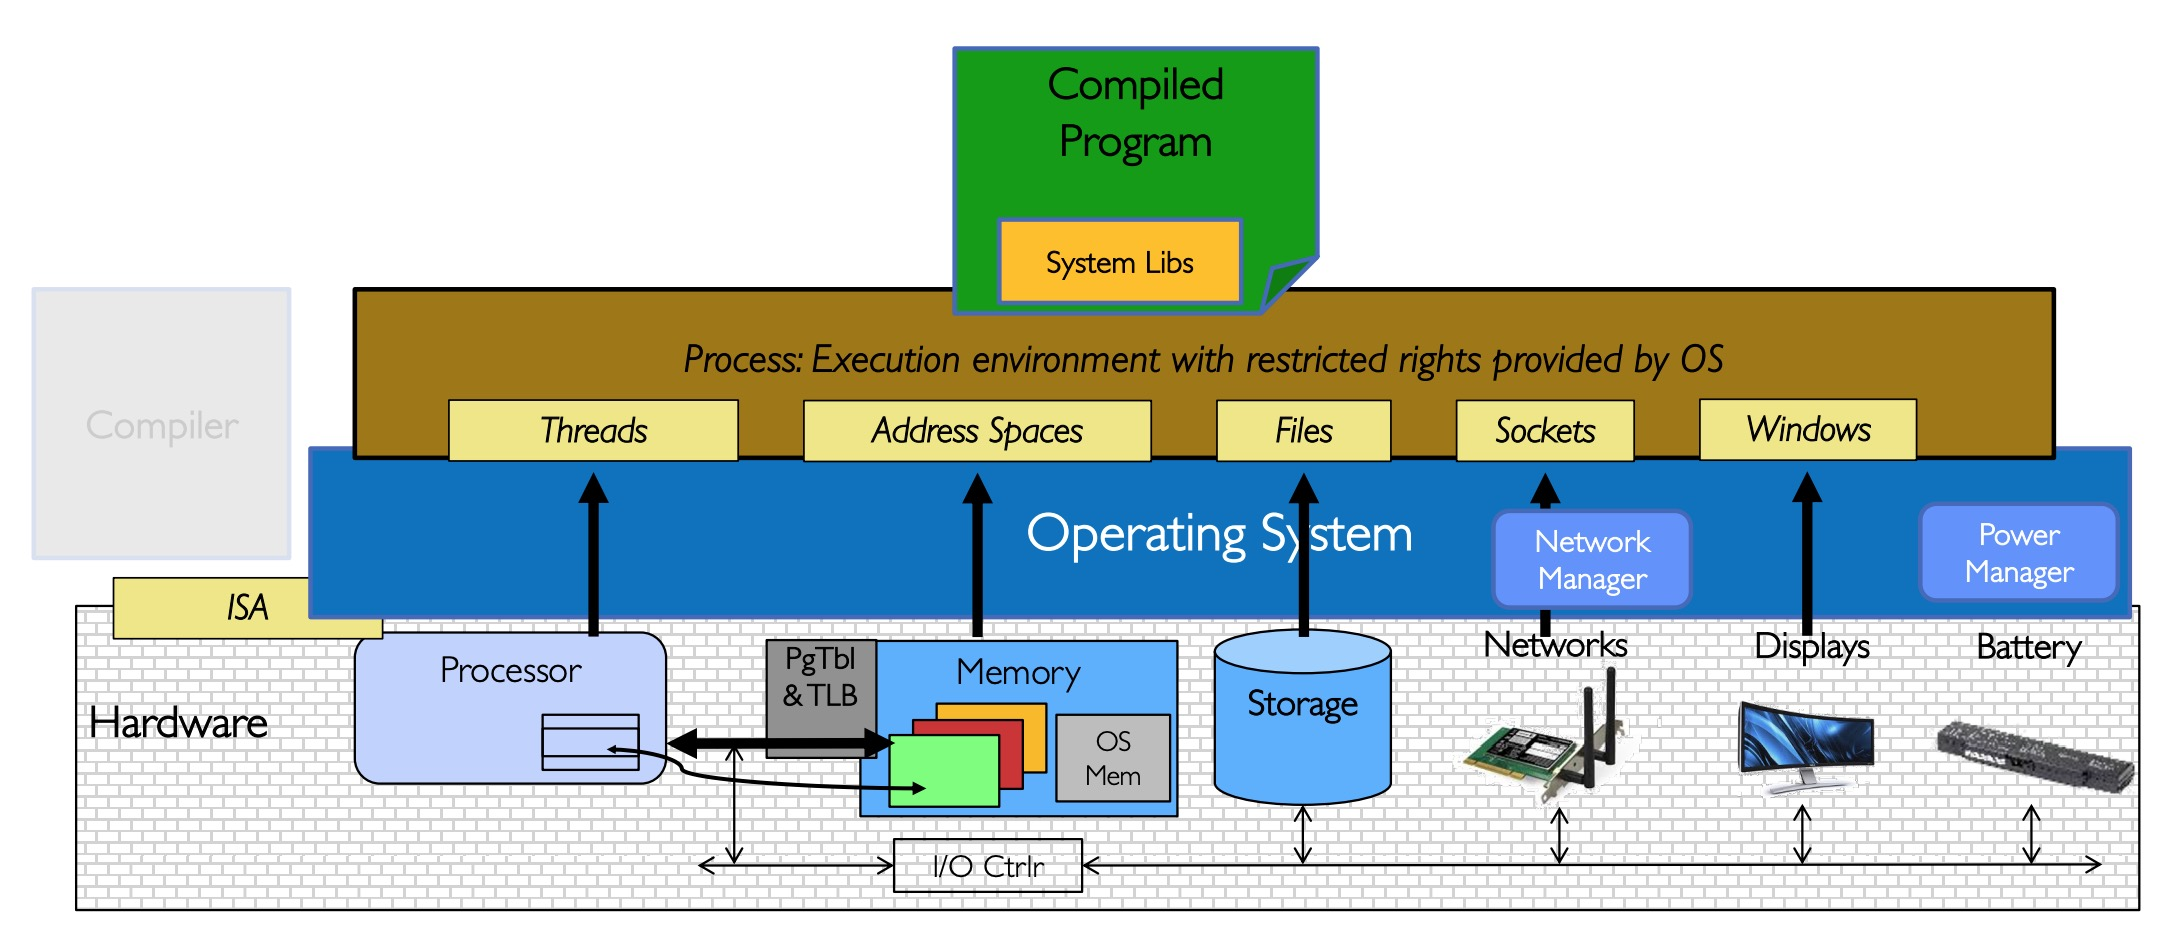
\includegraphics[width = 0.8\textwidth ]{figures/background_management.jpg}
    \caption{Background Management}
    % \label{fig:batteryIncreas}
\end{figure}

\begin{tcolorbox}
\begin{discussion}
How do we tame complexity?
\end{discussion}
\paragraph{Virtual Machine Abstraction} For software engineering Problem, system will turn hardware/software quirks to what programmers want/need
\begin{figure}[H]
    \centering
    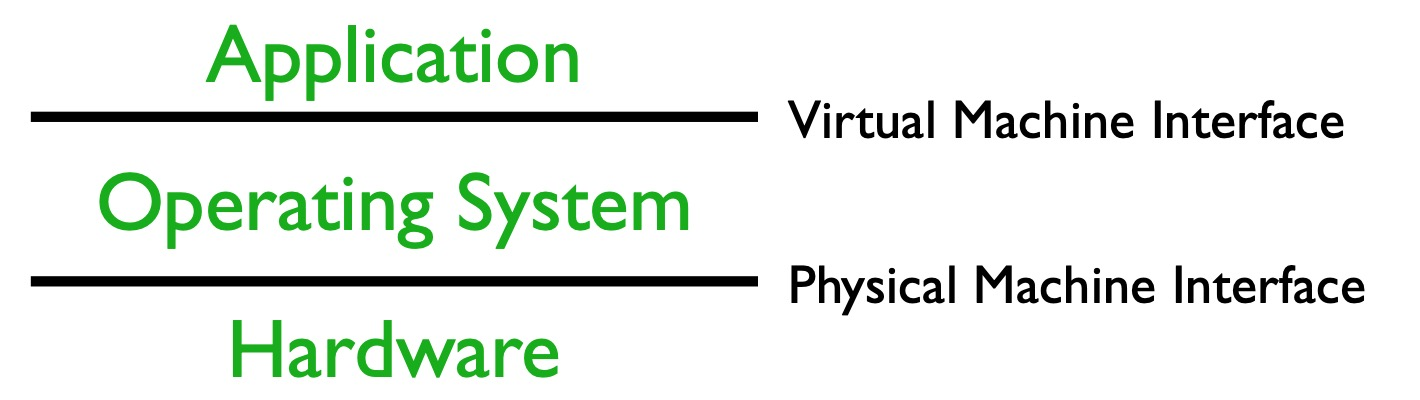
\includegraphics[width = 0.6\textwidth ]{figures/vma.jpg}
    \caption{Virtual Machine Abstraction}
    % \label{fig:batteryIncreas}
\end{figure}
\end{tcolorbox}

\subsection{Virtual Machine}
Two types of Virtual Machine:
\begin{itemize}
    \item \textbf{Process VM:} supports the execution of a single program; this functionality typically provided by OS
\item \textbf{System VM:} supports the execution of an entire OS and its applications (e.g.,
VMWare Fusion, Virtual box, Parallels Desktop, Xen)
\end{itemize}

\subsubsection{Process VMs}
\textbf{Programming simplicity}
\begin{itemize}
    \item Each process thinks it has \textbf{all} memory/CPU time
    \item Each process thinks it owns \textbf{all} devices
    \item Different devices appear to have \textbf{same} high level interface
    \item Device interfaces more powerful than raw hardware
\end{itemize}
\textbf{Fault Isolation}
\begin{itemize}
    \item Processes \textbf{unable} to\textbf{ directly impact other processes}
    \item Bugs \textbf{cannot} crash whole machine
\end{itemize}
\textbf{Protection and Portability}
\begin{itemize}
    \item Java interface safe and stable across many platforms
\end{itemize}

\subsubsection{System Virtual Machines: Layers of OSs}
Useful for OS development
\begin{itemize}
    \item When OS crashes, restricted to one VM
    \item Can aid testing programs on other OSs
\end{itemize}
\begin{figure}[H]
    \centering
    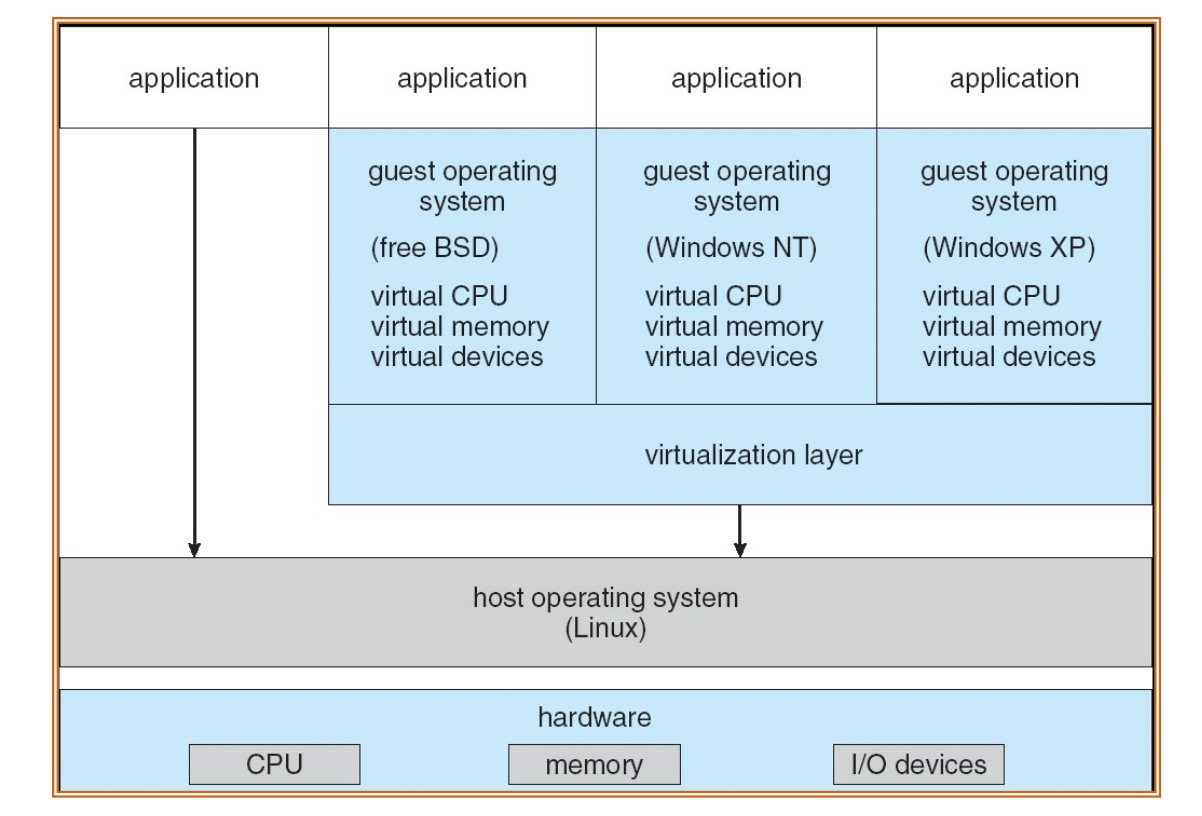
\includegraphics[width = 0.6\textwidth ]{figures/vm.jpg}
    \caption{Virtual Machine}
    % \label{fig:batteryIncreas}
\end{figure}



% \begin{figure}[H]
%     \centering
%     
\includegraphics[width = 0.8\textwidth ]{figures/tex.png}
%     \caption{Increase of battery capacity. }
%     \label{fig:batteryIncreas}
% \end{figure}


% In \autoref{tab:table1}

% \begin{table}[H]
%     \centering
%     \caption{That is a table.}
%     \begin{tabular}{|c|c|c|}
%     \centering
%     \textbf{Lorem} & \textbf{Ipsum} & \textbf{Lorem [\$]} \\ \hline \hline
% 1   & lipsum    & lorem     \\ \hline   
% 2   & lipsum    & lorem   \\ \hline
% 3   & lipsum    & lorem  
%     \end{tabular}
%     \label{tab:table1}
% \end{table}

